% =========================================================
% BEATRIZ VOCURCA FRADE
% ATS / AI FRIENDLY BILINGUAL RESUME — shared preamble + content
%
% Build (pdfLaTeX, run twice):
%   pdflatex resume-en.tex
%   pdflatex resume-pt.tex
%
% Bullets follow the STAR method (Situation, Task, Action, Result),
% compressed into "context -> action -> result" sentences.
% =========================================================

\documentclass[10pt,a4paper]{article}

% =========================================================
% PACKAGES
% =========================================================
\usepackage[
    top=0.85cm,
    bottom=0.85cm,
    left=1.15cm,
    right=1.15cm
]{geometry}

\usepackage[T1]{fontenc}
\usepackage[utf8]{inputenc}
\usepackage{lmodern}
\usepackage{microtype}
\usepackage{xcolor}
\usepackage{graphicx}
\usepackage{fontawesome5}
\usepackage{enumitem}
\usepackage{tabularx}
\usepackage{array}
\usepackage{hyperref}
\usepackage{ragged2e}
\usepackage{needspace}
\usepackage{ifthen}

% Improves PDF text extraction for ATS / AI systems
\input{glyphtounicode}
\pdfgentounicode=1

% ATS: icons are decorative. Map every icon glyph to a plain space so text
% extractors (pdftotext, PDFBox, Tika...) never emit stray characters next to
% contact details or section headings.
\pdfglyphtounicode{map-marker-alt}{0020}
\pdfglyphtounicode{envelope}{0020}
\pdfglyphtounicode{linkedin}{0020}
\pdfglyphtounicode{github}{0020}
\pdfglyphtounicode{user}{0020}
\pdfglyphtounicode{code}{0020}
\pdfglyphtounicode{briefcase}{0020}
\pdfglyphtounicode{rocket}{0020}
\pdfglyphtounicode{graduation-cap}{0020}
\pdfglyphtounicode{language}{0020}

% ATS: write real space characters into the PDF text layer. Without this some
% parsers (e.g. pypdf) glue words at font changes ("inFlutter", "merged500+"),
% which breaks keyword matching.
\pdfinterwordspaceon

% =========================================================
% GLOBAL CONFIGURATION
% =========================================================
\pagestyle{empty}

\setlength{\parindent}{0pt}
\setlength{\parskip}{0pt}

\renewcommand{\familydefault}{\sfdefault}

\clubpenalty=10000
\widowpenalty=10000

% ATS: never hyphenate, so keywords (e.g. "Flutter", "WebSocket") are never
% split across lines in the extracted text.
\hyphenpenalty=10000
\exhyphenpenalty=10000
\emergencystretch=2em

% =========================================================
% COLORS
% =========================================================
\definecolor{primary}{HTML}{223846}
\definecolor{accent}{HTML}{3F6678}
\definecolor{muted}{HTML}{66747D}
\definecolor{text}{HTML}{20252A}
\definecolor{line}{HTML}{CDD7DC}
\definecolor{soft}{HTML}{F3F6F7}
\definecolor{white}{HTML}{FFFFFF}

% =========================================================
% PERSONAL INFORMATION
% (phone intentionally omitted from the public version)
% =========================================================
\newcommand{\FullName}{Beatriz Vocurca Frade}

\newcommand{\Email}
{beatrizvocurcafrade@gmail.com}

\newcommand{\LinkedInURL}
{https://www.linkedin.com/in/beatriz-mobile/}

\newcommand{\LinkedInText}
{linkedin.com/in/beatriz-mobile}

\newcommand{\GitHubURL}
{https://github.com/BeatrizVocurcaFrade}

\newcommand{\GitHubText}
{github.com/BeatrizVocurcaFrade}

\newcommand{\LocationEN}
{Belo Horizonte, Minas Gerais, Brazil}

\newcommand{\LocationPT}
{Belo Horizonte, Minas Gerais, Brasil}

\newcommand{\CollectorURL}
{https://pub.dev/packages/collector_flutter}

\newcommand{\RoadsURL}
{https://github.com/BeatrizVocurcaFrade/trabalho_rp}

% =========================================================
% PDF / LINKS
% =========================================================
\hypersetup{
    colorlinks=true,
    urlcolor=accent,
    linkcolor=accent,
    pdfauthor={Beatriz Vocurca Frade},
    pdftitle={
        Beatriz Vocurca Frade - Mobile Software Engineer - Flutter Developer
    },
    pdfsubject={
        Mobile Software Engineering, Flutter and Software Development Resume
    },
    pdfkeywords={
        Flutter,
        Dart,
        Flutter Developer,
        Mobile Developer,
        Mobile Software Engineer,
        Software Engineer,
        Mobile Engineer,
        BLoC,
        go\_router,
        freezed,
        gRPC,
        WebSocket,
        Firebase,
        React,
        React Native,
        Java,
        Spring,
        AWS,
        AWS CDK,
        AWS Lambda,
        Amazon SQS,
        Python,
        REST API,
        REST APIs,
        API Integration,
        Clean Architecture,
        Clean Code,
        Performance Monitoring,
        Open Source,
        pub.dev,
        Git,
        GitHub,
        GitHub Actions,
        Azure DevOps,
        Figma,
        Swagger,
        Automated Testing,
        Unit Testing,
        Widget Testing,
        Code Review,
        Refactoring,
        Debugging,
        Agile,
        Scrum,
        Kanban,
        Football,
        Sports Data,
        Football Statistics,
        Sports Betting
    }
}

\urlstyle{same}

% =========================================================
% LIST CONFIGURATION
% =========================================================
\setlist[itemize]{
    leftmargin=0.43cm,
    itemsep=0.035cm,
    topsep=0.055cm,
    parsep=0pt,
    partopsep=0pt
}

% =========================================================
% SECTION
% =========================================================
\newcommand{\cvsection}[2]{

    \needspace{4\baselineskip}

    \vspace{0.18cm}

    {\large
    \bfseries
    \color{primary}
    #1
    \hspace{0.10cm}
    #2}

    \vspace{0.025cm}

    {\color{line}
    \rule{\linewidth}{0.65pt}}

    \vspace{0.07cm}
}

% =========================================================
% EXPERIENCE
% =========================================================
\newcommand{\experience}[4]{

    \needspace{5\baselineskip}

    \begin{tabularx}{\linewidth}{
        @{}
        >{\raggedright\arraybackslash}X
        >{\raggedleft\arraybackslash}p{3.25cm}
        @{}
    }

    {\bfseries\color{text}#1}
    &
    {\small\bfseries\color{accent}#3}

    \\[-0.01cm]

    {\small
    \bfseries
    \color{muted}
    #2}
    &

    \end{tabularx}

    \vspace{-0.09cm}

    {\small
    \color{text}
    #4
    }

    \vspace{0.07cm}
}

% =========================================================
% EDUCATION
% =========================================================
\newcommand{\education}[4]{

    \needspace{3\baselineskip}

    \begin{tabularx}{\linewidth}{
        @{}
        >{\raggedright\arraybackslash}X
        >{\raggedleft\arraybackslash}p{3.1cm}
        @{}
    }

    {\bfseries\color{text}#1}
    &
    {\small\bfseries\color{accent}#3}

    \\[-0.01cm]

    {\small\color{muted}#2}
    &

    \end{tabularx}

    \ifthenelse{\equal{#4}{}}
    {}
    {
        {\small\color{text}#4}
    }

    \vspace{0.09cm}
}

% =========================================================
% PROJECT
% =========================================================
\newcommand{\project}[3]{

    \needspace{2\baselineskip}

    {\small
    \textbf{\color{text}#1}
    \hspace{0.06cm}
    {\color{muted}|}
    \hspace{0.06cm}
    {\color{accent}#2}

    \vspace{0.02cm}

    \color{text}
    #3
    }

    \vspace{0.08cm}
}

% =========================================================
% SKILL LINE
% =========================================================
\newcommand{\skillline}[2]{
    {\small
    \textbf{\color{primary}#1:}
    \color{text}
    #2
    }

    \vspace{0.045cm}
}

% =========================================================
% HEADER
% =========================================================
\newcommand{\CVHeader}[3]{

    \noindent
    \begin{tabularx}{\linewidth}{
        @{}
        >{\raggedright\arraybackslash}X
        >{\centering\arraybackslash}p{4.45cm}
        @{}
    }

    % =====================================================
    % LEFT SIDE
    % =====================================================
    \begin{minipage}[c]{\linewidth}

        {\fontsize{24}{27}\selectfont
        \bfseries
        \color{primary}
        \FullName}

        \vspace{0.045cm}

        {\normalsize
        \bfseries
        \color{accent}
        #1}

        \vspace{0.055cm}

        {\small
        \color{muted}
        #2}

        \vspace{0.15cm}

        {\small
        \color{text}

        \faMapMarker*
        \hspace{0.045cm}
        #3
        \\[0.08cm]
        \faEnvelope
        \hspace{0.045cm}
        \href{mailto:\Email}{\Email}
        \\[0.08cm]
        \faLinkedin
        \hspace{0.045cm}
        \href{\LinkedInURL}{\LinkedInText}
        \\[0.08cm]
        \faGithub
        \hspace{0.045cm}
        \href{\GitHubURL}{\GitHubText}

        }

    \end{minipage}

    &

    % =====================================================
    % PROFILE PHOTO (profile.jpg next to this file)
    % =====================================================
    \begin{minipage}[c]{4.45cm}

        \centering

        \IfFileExists{profile.jpg}
        {
            \fcolorbox{line}{white}{%
                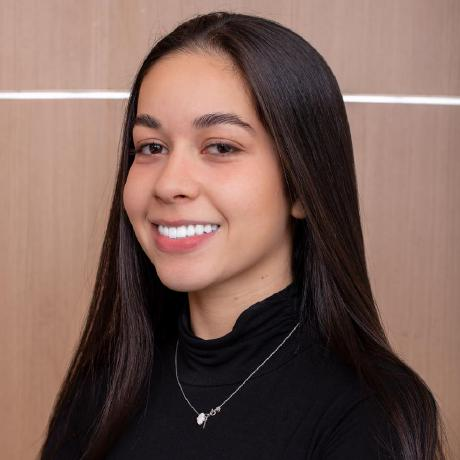
\includegraphics[
                    width=4.20cm,
                    height=4.20cm,
                    keepaspectratio
                ]{profile.jpg}%
            }
        }
        {
            \fcolorbox{line}{soft}{
                \parbox[c][4.20cm][c]{4.20cm}{
                    \centering

                    \color{muted}

                    \Large
                    \faUser

                    \\[0.10cm]

                    \scriptsize
                    profile.jpg
                }
            }
        }

    \end{minipage}

    \end{tabularx}

    \vspace{0.10cm}

    {\color{primary}
    \rule{\linewidth}{1.15pt}}

    \vspace{0.10cm}
}

% =========================================================
% =========================================================
% ENGLISH VERSION
% =========================================================
% =========================================================

\newcommand{\EnglishCV}{

\CVHeader
{MOBILE SOFTWARE ENGINEER \;|\; FLUTTER DEVELOPER}
{Systems Engineering \;•\; Mobile Development \;•\; Software Engineering}
{\LocationEN}

% =========================================================
% SUMMARY
% =========================================================
\cvsection{\faUser}{Professional Summary}

{\small
\justifying
Mobile Software Engineer specialized in \textbf{Flutter and Dart}, building
\textbf{R10 Score}, a football live-scores and statistics app with
\textbf{1M+ downloads} on Google Play. In a production Flutter monorepo I have
merged \textbf{500+ pull requests} and performed \textbf{570+ code reviews},
delivering features end to end, from Figma and API contracts to tested releases
on both stores. Author of \textbf{collector\_flutter}, an open-source
performance-monitoring package published on pub.dev.

Background in Systems Engineering (UFMG) and hands-on experience with
\textbf{React, React Native, Java and Spring}. I work closely with
product, design, backend and QA teams in agile environments, with a strong
focus on clean architecture, automated testing and root-cause debugging.
}

% =========================================================
% CORE SKILLS
% =========================================================
\cvsection{\faCode}{Technical Skills}

\skillline
{Mobile Development}
{Flutter, Dart, Android, iOS, BLoC, go\_router, freezed, Firebase, React Native}

\skillline
{Real-time \& APIs}
{REST APIs, JSON, gRPC streaming, WebSocket, Swagger / OpenAPI}

\skillline
{Frontend Development}
{React, responsive interfaces, reusable UI components, design systems}

\skillline
{Backend \& Cloud}
{Java, Spring, AWS CDK, AWS Lambda, Amazon SQS, MongoDB}

\skillline
{Programming Languages \& Data}
{Dart, Java, JavaScript, TypeScript, Python, C, C++, SQL}

\skillline
{Architecture \& Engineering}
{Clean Architecture, Clean Code, modular monorepos, refactoring,
performance monitoring}

\skillline
{Software Quality}
{Unit, widget and BLoC tests (mocktail, bloc\_test), Code Review,
debugging, static analysis, Software Security}

\skillline
{Delivery \& Collaboration}
{Git, GitHub, GitHub Actions, CI/CD, Azure DevOps, Figma, Pull Requests,
Scrum, Kanban, Agile}

% =========================================================
% EXPERIENCE
% =========================================================
\cvsection{\faBriefcase}{Professional Experience}

\experience
{Mobile Software Developer | Flutter Developer}
{R10 Score | OTG VENTURES LTDA}
{May 2025 -- Present}
{
\begin{itemize}

    \item
    Build and maintain \textbf{R10 Score}, a football live-scores, statistics
    and betting-tips app with \textbf{1M+ Google Play downloads} and a
    \textbf{4.5-star App Store rating}, in a Flutter monorepo with 11 packages
    (BLoC, go\_router, freezed, REST, gRPC and WebSocket).

    \item
    Merged \textbf{500+ pull requests} and performed \textbf{570+ code
    reviews} across the mobile app, backend hub and architecture-docs
    repositories, under strict static-analysis rules.

    \item
    Delivered the \textbf{Mural bet-wall tab}, a drag-and-drop ticket grid
    with backend-persisted order and live WebSocket updates, splitting a
    148-file feature into 5 stacked, independently reviewable pull requests.

    \item
    Built the \textbf{2026 World Cup experience} (CMS-driven tabs, paginated
    guess leaderboard, match and team headers) across \textbf{49 merged pull
    requests} for the tournament period.

    \item
    When Google Play began rejecting uploads after the August 2026
    target-API deadline, raised targetSdk to 36 and upgraded Play Billing
    Library to 8.0.0, \textbf{unblocking store publishing} for the next
    release.

    \item
    Traced an intermittent freeze in match-statistics navigation to
    \textbf{two independent root causes} (an animation/state race and a
    subtree remount), fixed both and added timing-based regression tests.

    \item
    Restored the app test suite from 8 failing to \textbf{388/388 passing}
    by fixing 3 root causes, including 2 real production bugs in splash
    navigation and BLoC state handling.

    \item
    Validate API contracts with backend (Swagger), turn Figma specs into
    reusable components with design, and prepare releases with QA and
    product in Azure DevOps; also contribute to Tylty and React web
    projects.
\end{itemize}
}

\experience
{Programming Instructor}
{Garotas Aplicadas Project -- AVEC | Centro Universitário Una}
{2024 -- 2025}
{
\begin{itemize}

    \item
    To widen female participation in technology, taught theory and hands-on
    programming classes to public high-school girls from Belo Horizonte and
    its metropolitan region, turning technical concepts into accessible
    lessons.

    \item
    Supported entrepreneurship, career-development and professional
    preparation activities, helping participants build both technical and
    interpersonal skills.
\end{itemize}
}

\experience
{Mobile Developer -- Freelance}
{Drum Coach | International Project -- Germany}
{2025}
{
\begin{itemize}

    \item
    Built an interactive \textbf{Flutter and Dart} app that helps musicians
    and beginners learn and practice drums, with responsive, dynamic
    interfaces designed for an engaging learning experience.

    \item
    Delivered autonomously while collaborating remotely with an international
    team, strengthening distributed development and technical communication.
\end{itemize}
}

\experience
{Mobile Developer}
{Prime Results}
{2022 -- 2025}
{
\begin{itemize}

    \item
    Delivered mobile features end to end in \textbf{Flutter and Dart}, from
    \textbf{Figma} specifications through \textbf{REST API} integration,
    testing and release.

    \item
    Worked across the stack, contributing to backend services in
    \textbf{Java and Spring} and to \textbf{React} web projects.

    \item
    Applied \textbf{Clean Code and Clean Architecture} principles and took
    part in code reviews, automated testing and security practices, making
    the codebases easier to maintain, scale and evolve.
\end{itemize}
}

\experience
{Business Analyst \& Front-End Developer}
{iJunior}
{2021 -- 2022}
{
\begin{itemize}

    \item
    Worked with clients and the sales team to gather business requirements
    and translate them into viable digital solutions, bridging business and
    technology.

    \item
    Built customized apps and websites with \textbf{React Native} and
    frontend technologies for organizations across different sectors, using
    \textbf{Scrum and Kanban} for iterative delivery.
\end{itemize}
}

\experience
{Systems Analyst}
{Interact Place}
{2020 -- 2021}
{
\begin{itemize}

    \item
    Helped build an interactive mobile exhibition guide for
    \textbf{Palácio das Artes}, one of Belo Horizonte's major cultural
    institutions, where QR codes connect visitors to information about
    artworks, making cultural content more accessible and engaging.
\end{itemize}
}

% =========================================================
% PROJECTS
% =========================================================
\cvsection{\faRocket}{Projects}

\project
{collector\_flutter}
{\href{\CollectorURL}{pub.dev/packages/collector\_flutter}}
{Open-source Flutter plugin for real-time performance monitoring (FPS,
jank, memory, CPU, battery, HTTP traffic and custom events) with an in-app
dashboard and heuristic recommendations, built with Clean Architecture.
Published on pub.dev with \textbf{150/160 pub points}; developed as my
undergraduate thesis at UFMG.}

\project
{Road Network Detection}
{\href{\RoadsURL}{github.com/BeatrizVocurcaFrade/trabalho\_rp}}
{Team project (UFMG Pattern Recognition): Python computer-vision pipeline
that detects roads in satellite images with color and texture cues, a Frangi
ridge filter and oriented morphology, and explores graph reconstruction of
the road network.}

% =========================================================
% EDUCATION
% =========================================================
\cvsection{\faGraduationCap}{Education}

\education
{Bachelor's Degree in Systems Engineering}
{Federal University of Minas Gerais -- UFMG}
{2020 -- 2026}
{Thesis: Monitoring and Optimizing Resource Consumption in Flutter Apps
(collector\_flutter), advised by Prof. Ramon Lacerda Marques.}

\education
{High School}
{Colégio Nossa Senhora das Dores}
{2014 -- 2019}
{}

% =========================================================
% LANGUAGES
% =========================================================
\cvsection{\faLanguage}{Languages}

\skillline
{Portuguese}
{Native}

\skillline
{English}
{TOEFL certified; English language program at CCAA -- Floresta (2008 -- 2019)}

}

% =========================================================
% =========================================================
% PORTUGUESE VERSION
% =========================================================
% =========================================================

\newcommand{\PortugueseCV}{

\CVHeader
{ENGENHEIRA DE SOFTWARE MOBILE \;|\; DESENVOLVEDORA FLUTTER}
{Engenharia de Sistemas \;•\; Desenvolvimento Mobile \;•\; Engenharia de Software}
{\LocationPT}

% =========================================================
% SUMMARY
% =========================================================
\cvsection{\faUser}{Resumo Profissional}

{\small
\justifying
Engenheira de Software Mobile especializada em \textbf{Flutter e Dart},
desenvolvendo o \textbf{R10 Score}, aplicativo de resultados ao vivo e
estatísticas de futebol com \textbf{mais de 1 milhão de downloads} no Google
Play. Em um monorepo Flutter em produção, já tive \textbf{mais de 500 pull
requests mergeados} e fiz \textbf{mais de 570 code reviews}, entregando
funcionalidades de ponta a ponta, do Figma e dos contratos de API até
releases testadas nas duas lojas. Autora do \textbf{collector\_flutter},
pacote open source de monitoramento de desempenho publicado no pub.dev.

Formação em Engenharia de Sistemas (UFMG) e experiência prática com
\textbf{React, React Native, Java e Spring}. Trabalho em conjunto com
equipes de produto, design, backend e QA em ambientes ágeis, com foco em
arquitetura limpa, testes automatizados e investigação de causa raiz.
}

% =========================================================
% CORE SKILLS
% =========================================================
\cvsection{\faCode}{Competências Técnicas}

\skillline
{Desenvolvimento Mobile}
{Flutter, Dart, Android, iOS, BLoC, go\_router, freezed, Firebase, React Native}

\skillline
{Tempo Real \& APIs}
{APIs REST, JSON, streaming gRPC, WebSocket, Swagger / OpenAPI}

\skillline
{Desenvolvimento Frontend}
{React, interfaces responsivas, componentes reutilizáveis, design systems}

\skillline
{Backend \& Cloud}
{Java, Spring, AWS CDK, AWS Lambda, Amazon SQS, MongoDB}

\skillline
{Linguagens \& Dados}
{Dart, Java, JavaScript, TypeScript, Python, C, C++, SQL}

\skillline
{Arquitetura \& Engenharia}
{Clean Architecture, Clean Code, monorepos modulares, refatoração,
monitoramento de desempenho}

\skillline
{Qualidade de Software}
{Testes unitários, de widget e de BLoC (mocktail, bloc\_test), Code Review,
debugging, análise estática, Segurança de Software}

\skillline
{Entrega \& Colaboração}
{Git, GitHub, GitHub Actions, CI/CD, Azure DevOps, Figma, Pull Requests,
Scrum, Kanban, Metodologias Ágeis}

% =========================================================
% EXPERIENCE
% =========================================================
\cvsection{\faBriefcase}{Experiência Profissional}

\experience
{Desenvolvedora de Software Mobile | Flutter Developer}
{R10 Score | OTG VENTURES LTDA}
{Mai 2025 -- Atual}
{
\begin{itemize}

    \item
    Desenvolvimento e manutenção do \textbf{R10 Score}, aplicativo de
    resultados ao vivo, estatísticas e palpites de futebol com \textbf{mais
    de 1 milhão de downloads no Google Play} e \textbf{nota 4,5 na App
    Store}, em um monorepo Flutter com 11 pacotes (BLoC, go\_router, freezed,
    REST, gRPC e WebSocket).

    \item
    \textbf{Mais de 500 pull requests mergeados} e \textbf{mais de 570 code
    reviews} nos repositórios do app mobile, do backend hub e da
    documentação de arquitetura, sob regras rígidas de análise estática.

    \item
    Entrega da \textbf{aba Mural de apostas}, um grid de bilhetes com
    arrastar e soltar, ordem salva no backend e atualização ao vivo via
    WebSocket, dividindo uma feature de 148 arquivos em 5 pull requests
    empilhados e revisáveis de forma independente.

    \item
    Construção da \textbf{experiência da Copa do Mundo 2026} (abas via CMS,
    ranking de palpites paginado, cabeçalhos de partidas e seleções) em
    \textbf{49 pull requests mergeados}, para o período do torneio.

    \item
    Quando o Google Play passou a rejeitar uploads após o prazo de API alvo
    de agosto de 2026, atualização do targetSdk para 36 e da Play Billing
    Library para 8.0.0, \textbf{destravando a publicação} da release
    seguinte.

    \item
    Investigação de um travamento intermitente na navegação das estatísticas
    de partida até \textbf{duas causas raiz independentes} (uma race entre
    animação e estado e um remount de subárvore), com correção de ambas e
    testes de regressão baseados em timing.

    \item
    Recuperação da suíte de testes do app, de 8 falhas para \textbf{388/388
    passando}, corrigindo 3 causas raiz, entre elas 2 bugs reais de produção
    na navegação do splash e no estado de um BLoC.

    \item
    Validação de contratos de API com o backend (Swagger), transformação de
    specs do Figma em componentes reutilizáveis com o design e preparação de
    releases com QA e produto no Azure DevOps; contribuição também com o
    Tylty e projetos web em React.
\end{itemize}
}

\experience
{Instrutora de Programação}
{Projeto Garotas Aplicadas -- AVEC | Centro Universitário Una}
{2024 -- 2025}
{
\begin{itemize}

    \item
    Aulas teóricas e práticas de programação para estudantes do ensino
    médio da rede pública de Belo Horizonte e Região Metropolitana, com o
    objetivo de ampliar a participação feminina na tecnologia.

    \item
    Apoio a atividades de empreendedorismo e preparação profissional das
    participantes.
\end{itemize}
}

\experience
{Desenvolvedora Mobile -- Freelancer}
{Drum Coach | Projeto Internacional -- Alemanha}
{2025}
{
\begin{itemize}

    \item
    Aplicativo interativo em \textbf{Flutter e Dart} para músicos e
    iniciantes aprenderem e praticarem bateria, com interfaces responsivas
    e dinâmicas focadas em uma aprendizagem envolvente.

    \item
    Entregas autônomas em colaboração remota com equipe internacional.
\end{itemize}
}

\experience
{Desenvolvedora Mobile}
{Prime Results}
{2022 -- 2025}
{
\begin{itemize}

    \item
    Entrega de funcionalidades mobile de ponta a ponta em \textbf{Flutter e
    Dart}, do \textbf{Figma} às \textbf{APIs REST}, testes e release.

    \item
    Atuação em toda a stack, contribuindo com serviços backend em
    \textbf{Java e Spring} e com projetos web em \textbf{React}.

    \item
    Aplicação de \textbf{Clean Code e Clean Architecture} e participação em
    code reviews, testes automatizados e práticas de segurança, tornando o
    código mais fácil de manter, escalar e evoluir.
\end{itemize}
}

\experience
{Analista de Negócios \& Desenvolvedora Front-End}
{iJunior}
{2021 -- 2022}
{
\begin{itemize}

    \item
    Levantamento de requisitos com clientes e equipe comercial, traduzindo
    necessidades de negócio em soluções digitais viáveis.

    \item
    Desenvolvimento de aplicações e sites personalizados com \textbf{React
    Native} e tecnologias frontend para organizações de diferentes
    segmentos, com \textbf{Scrum e Kanban} para entregas iterativas.
\end{itemize}
}

\experience
{Analista de Sistemas}
{Interact Place}
{2020 -- 2021}
{
\begin{itemize}

    \item
    Participação no desenvolvimento de um guia de exposição mobile
    interativo para o \textbf{Palácio das Artes}, uma das principais
    instituições culturais de Belo Horizonte, com QR Codes que levam os
    visitantes às informações das obras.
\end{itemize}
}

% =========================================================
% PROJECTS
% =========================================================
\cvsection{\faRocket}{Projetos}

\project
{collector\_flutter}
{\href{\CollectorURL}{pub.dev/packages/collector\_flutter}}
{Plugin Flutter open source para monitoramento de desempenho em tempo real
(FPS, jank, memória, CPU, bateria, tráfego HTTP e eventos customizados), com
dashboard dentro do app e recomendações heurísticas, construído com Clean
Architecture. Publicado no pub.dev com \textbf{150/160 pub points};
desenvolvido como TCC na UFMG.}

\project
{Detecção de Malha Viária}
{\href{\RoadsURL}{github.com/BeatrizVocurcaFrade/trabalho\_rp}}
{Projeto em equipe (Reconhecimento de Padrões, UFMG): detecção de vias em
imagens de satélite em Python com cor, textura, filtro de Frangi e morfologia
orientada, explorando a malha viária como grafo.}

% =========================================================
% EDUCATION
% =========================================================
\cvsection{\faGraduationCap}{Formação Acadêmica}

\education
{Bacharelado em Engenharia de Sistemas}
{Universidade Federal de Minas Gerais -- UFMG}
{2020 -- 2026}
{TCC: Monitoramento e Otimização do Consumo de Recursos em Aplicativos
Flutter, orientado pelo Prof. Ramon Lacerda Marques.}

\education
{Ensino Médio}
{Colégio Nossa Senhora das Dores}
{2014 -- 2019}
{}

% =========================================================
% LANGUAGES
% =========================================================
\cvsection{\faLanguage}{Idiomas}

\skillline
{Português}
{Nativo}

\skillline
{Inglês}
{Certificação TOEFL; curso de inglês no CCAA -- Floresta (2008 -- 2019)}

}
